\section*{Task}

In 1978, an influenza epidemic (caused by the H1N1 virus) broke out in a boarding school
in Great Britain, where 763 pupils studied and lived. The epidemic affected more than
two-thirds of all the pupils (see Fig.~3). It began when the students returned to school
after the holidays—one of them arrived already ill. To stop the epidemic, each pupil who
developed a fever was immediately isolated from others and confined to bed as soon as the
first flu symptoms appeared. After a few days, their condition improved, and after several
more days they fully recovered.

The table below shows how, during the epidemic, the number of pupils who were ill
(confined to bed) and those who were recovering (convalescent) changed over time.

\begin{table}[h!]
\centering
\caption{Amount of ill and recovering pupils during the epidemic.}
\begin{tabular}{ccccccccccccccc}
\toprule
Day of epidemic
(counting from January 22) &
1 & 2 & 3 & 4 & 5 & 6 & 7 & 8 & 9 & 10 & 11 & 12 & 13 & 14 \\
\midrule
Number of ill pupils &
3 & 8 & 26 & 76 & 225 & 298 & 258 & 233 & 189 & 128 & 68 & 29 & 14 & 4 \\
Number of recovering pupils &
0 & 0 & 0 & 0 & 9 & 17 & 105 & 162 & 176 & 166 & 150 & 85 & 47 & 20 \\
\bottomrule
\end{tabular}
\end{table}

\begin{enumerate}
  \item Propose a model that is consistent with the statistical data presented in Table~4.
  
  \item Perform numerical simulation and show that, with appropriate adjustment of the
  model parameters, your model can indeed describe this data.
  
  \item Based on your model, determine:
  \begin{enumerate}
    \item How many pupils in total became ill (compare this calculated number with the
    actual value of 512)?
    
    \item On average, how much time passed between a pupil's infection and the appearance
    of the first symptoms of the disease?
    
    \item On average, how many days did an ill pupil spend confined to bed, and after how
    many additional days of improvement did they fully recover?
    
    \item On which day of the epidemic did the total number of infected pupils (both those
    newly infected but not yet showing symptoms and those already confined to bed) reach
    its peak, and what was this number?
  \end{enumerate}
  
  \item Analyze how vaccination could help prevent the epidemic. Calculate what fraction
  of unvaccinated pupils would become infected if $n\%$ of all pupils (for example, in the
  range from $10\%$ to $90\%$) had been vaccinated before returning to school.
\end{enumerate}

\newpage

\section*{Introduction}

In 1947 John von Neumann, remarked \textit{"truth is much too complicated to allow anything but approximations"}. Epidemic models reflect this idea with a wide variety of possible models. Some are much too simple like a birth/death model, while others, require machine learning algorithms, consiquently large datasets and thus are too complicated for such a task. Instead a stochastic SEICR model is chosen for this problem. This model divides the population into five possible categories:
 
\begin{enumerate}
    \item (S) Susceptible - population which is susceptible to the desease, in this case all of pupils
    \item (E) Exposed - these are the people who are exposed to the desease, we include this category since many epidemics have a latency period
    \item (I) Infectious - prople who are infected and are able to infect others
    \item (C) Convalescent - population which is ill, but recovering
    \item (R) Recovered - Final category of recovered people
\end{enumerate}


\section*{Mathematical Modeling}

Given these definitions is it then clear how we can create a continuous time markov chain which connects all these states:

\begin{tikzpicture}[
  node distance=2.6cm,
  >=Latex,
  every node/.style={font=\small},
  state/.style={draw, rounded corners, minimum width=1.6cm, minimum height=0.9cm, align=center}
]

\node[state] (S) {$S$\\(susceptible)};
\node[state, right =3cm of S] (E) {$E$\\(latent)};
\node[state, right of=E] (I) {$I$\\(ill)};
\node[state, right of=I] (C) {$C$\\(conval.)};
\node[state, right of=C] (R) {$R$\\(recovered)};

\draw[->, thick] (S) -- (E)
  node[midway, above] {$\displaystyle \beta\,\frac{(E+kI)}{N}\,S$};

\draw[->, thick] (E) -- (I)
  node[midway, above] {$\displaystyle \alpha E$};

\draw[->, thick] (I) -- (C)
  node[midway, above] {$\displaystyle \gamma I$};

\draw[->, thick] (C) -- (R)
  node[midway, above] {$\displaystyle \delta C$};

\end{tikzpicture}


First thing to notice is that the total number of pupils is conserved 

\begin{equation}
    N = S + E + I + C + R = {\rm \textit{const}}
\end{equation}

with $S$, $E$, $I$, $C$ and $R$ are number of pupils that are susceptible, exposed, infectious, convalescent and recovered accordingly. Then the state space is just

\begin{equation*}
    \mathcal{S} = \{ (s,e,i,c,r) \in \mathbb{N}^5 | s+e+i+c+r = N \}
\end{equation*}

and the state is simply a vector

\begin{equation*}
    X(t) = (S(t), E(t), I(t), C(t), R(t))
\end{equation*}

We know that the evolution of this state obeys the Markov property. The evolution of this state can be seen easily derived from the graphic above

\begin{align}
    \frac{dS}{dt} = - \lambda(t) S; \quad \frac{dE}{dt} = \lambda(t) &S - \alpha E; \quad \frac{dI}{dt} = \alpha E - \gamma I; \notag \\
    \frac{dC}{dt} = \gamma I - \delta C; &\quad \frac{dR}{dt} = \delta C. \label{eq:differential}
\end{align}

where we use a force of infection function $\lambda(t)$

\begin{equation*}
    \lambda (t) = \beta \frac{E(t) + k I(t)}{N} \quad k \in [ 0 , 1 )
\end{equation*}

From these equations we can read off the rates
\begin{itemize}\label{event rates}
    \item S $\rightarrow$ E \quad $a_1 = \beta \frac{E + kI}{N} S$
    \item E $\rightarrow$ I \quad $a_2 = \alpha E$
    \item I $\rightarrow$ C \quad $a_3 = \gamma I$
    \item C $\rightarrow$ R \quad $a_4 = \delta C$
\end{itemize}

with the total event rate being $a_0 = a_1 + a_2 + a_3 + a_4$. This allows to compute probabilities of certain events happening
\begin{equation}\label{event probabilities}
  P (\text{j event}) = \frac{a_j}{a_0}
\end{equation}

\section*{Modeling}

The modeling is done in two main steps. First we need to find out the parameter values for $\alpha, \beta, \gamma, \delta$ and then we can use Monte Carlo simulations with Gillespie algorithm. The paramer values are obtained by solving the set of differential equations (\ref{eq:differential}) and optimising the solutions to fit the given data with pythons \texttt{scipy.optimize} library. We use least squares optimisation method which computes the error as follows

\begin{equation*}
    {\rm error} = \sum_t (I_{\rm model}(t) - I_{\rm obs})^2 + \sum_t (C_{\rm model}(t) - C_{\rm obs}(t))^2
\end{equation*}

where the indicies "model" and "obs" are the models and observed quantities correspondingly. Thus we obtain the following values

\begin{lstlisting}
beta   = 5.8866
alpha  = 3.1004
gamma  = 0.4983
delta  = 0.5948
\end{lstlisting}

To capture the stochastic nature of the model we use the aformentioned monte carlo simulation with the Gillespie algorithm. The algorithm works in the following way:

\begin{enumerate}
  \item Initialise the variables
  \item Loop while $t < T$
  \begin{itemize}
    \item Compute event rates (\ref{event rates}) and the total rate $a_0$
    \item Get random waiting time with $\delta t \sim \exp(a_0)$
    \item Update time $t \leftarrow t + \delta t$
    \item Pick random event using probabilities (\ref{event probabilities})
    \item Update the state
  \end{itemize}
  \item Return the recorded array of states
\end{enumerate}

Each simulation produces one possible epidemic realization, and by running many such simulations we can then compute the mean values. 

\begin{enumerate}[label=(\alph*)]
  \item Total ever became ill (stochastic mean) = 543.0 pupils
  \item Mean infection to symptoms = $1/\alpha = 0.323$ days
  \item Mean days ill in bed = $1/\gamma = 2.007$ days\\
        Mean extra convalescent = $1/\delta = 1.681$ days
  \item Peak of (E+I) deterministic: day 6.60, size 363.9
\end{enumerate}

\begin{figure}[h]
  \centering
  \begin{subfigure}{0.48\textwidth}
    \centering
    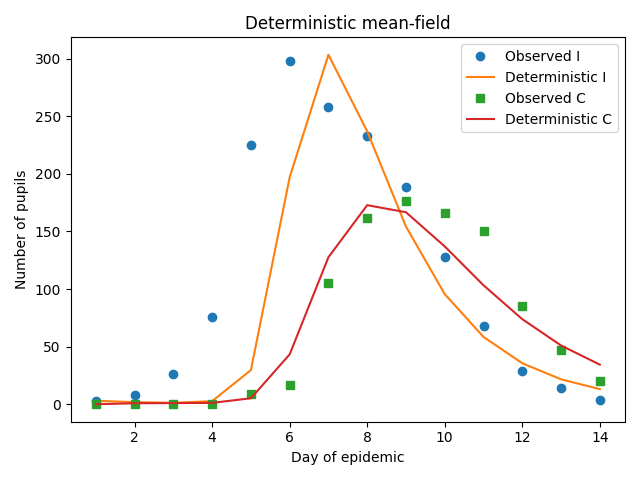
\includegraphics[width=\textwidth]{content/Figure_deterministic.png}
    \caption{Deterministic SEICR fit}
  \end{subfigure}
  \hfill
  \begin{subfigure}{0.48\textwidth}
    \centering
    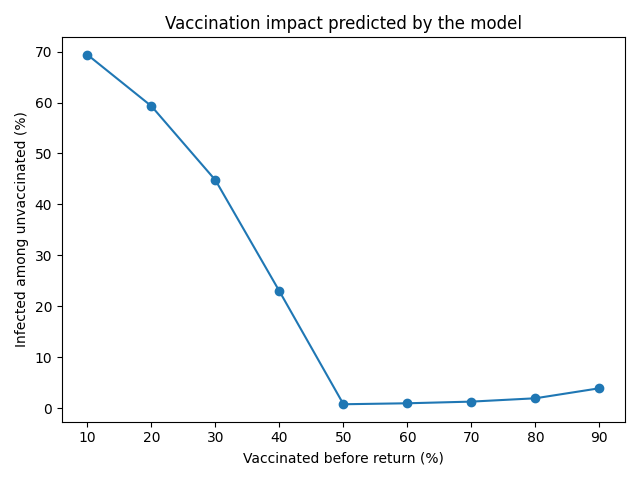
\includegraphics[width=\textwidth]{content/Figure_vaccination.png}
    \caption{Vaccination impact}
  \end{subfigure}
  \caption{SEICR epidemic model results for pupil outbreak}
\end{figure}


We can also plot the results. Figure 1 (a) shows how the deterministic SEICR model captured the outbreak shape. In general the model reproduces the order of magnitude and general evolution ill (I) and Convalescent (C) pupils. However, the peak if shifted and the early growth of infections is later than the observed data. Much of the discrepency can be attributed to the simplied model used: constant parameters, imperfect knowledge of initial conditions (especially initial latent infections) and most importantly the fact that the deterministic model reflects the \textit{average} behaviour, while the true outbreak is a stochastic process. Figure 2 (b) shows the vaccination impact curve which has a non trivial tendancies. For vaccination levels under $30 \%-40 \%$ the majority of the population still becomes infected. After increasing the number of vaccinated pupils to about $50 \%$ of pupils, the model shows a sharp drop in outbreak size. Beyond this threshold, a heard immunity has formed and further vaccination provides neglegible results.
